\documentclass[12pt,twoside]{book}

\usepackage{mathptm,times,color}
\usepackage[pdftex]{graphicx}
\usepackage{multirow}
\usepackage{bezier}
\usepackage{rotating}
\usepackage{longtable}
\usepackage{amsmath}
\usepackage{xfrac}
\usepackage{array}
\usepackage{units}
\usepackage{fix-cm}
\usepackage{xspace}
\usepackage{makeidx} % Create index at end of document
\usepackage[nottoc,notlof,notlot]{tocbibind} % Put the bibliography and index in the ToC
\usepackage{datetime}
\newdateformat{mydate}{\monthname[\THEMONTH] \THEYEAR}

\usepackage{listings}
\usepackage{textcomp}
\definecolor{lbcolor}{rgb}{0.96,0.96,0.96}
\lstset{
    %backgroundcolor=\color{lbcolor},
    tabsize=4,
    rulecolor=,
    language=Fortran,
        basicstyle=\footnotesize\ttfamily,
        upquote=true,
        aboveskip={\baselineskip},
        belowskip={\baselineskip},
        columns=fixed,
        extendedchars=true,
        breaklines=true,
        breakatwhitespace=true,
        frame=none,
        showtabs=false,
        showspaces=false,
        showstringspaces=false,
        identifierstyle=\ttfamily,
        keywordstyle=\color[rgb]{0,0,0},
        commentstyle=\color[rgb]{0,0,0},
        stringstyle=\color[rgb]{0,0,0},
}

\usepackage{wrapfig}
\usepackage{morefloats}

\newcolumntype{L}[1]{>{\raggedright\let\newline\\\arraybackslash\hspace{0pt}}m{#1}}
\newcolumntype{C}[1]{>{\centering\let\newline\\\arraybackslash\hspace{0pt}}m{#1}}
\newcolumntype{R}[1]{>{\raggedleft\let\newline\\\arraybackslash\hspace{0pt}}m{#1}}

\IfFileExists{../Bibliography/gitrevision.tex}
{\input{../Bibliography/gitrevision}}
{\newcommand{\gitrevision}{unknown} }

\usepackage{framed}
\newcommand{\graybox}[1]{
\begin{shaded}#1\end{shaded}
}

\usepackage{changepage}

\renewcommand{\bibname}{References}

% dummy change to force revision update

%\usepackage{eso-pic}
%\usepackage{graphicx}
%\usepackage{color}
%\usepackage{type1cm}


%\makeatletter
%   \AddToShipoutPicture{%
%     \setlength{\@tempdimb}{.5\paperwidth}%
%    \setlength{\@tempdimc}{.5\paperheight}%
%   \setlength{\unitlength}{1pt}%
%  \put(\strip@pt\@tempdimb,\strip@pt\@tempdimc){%
%     \makebox(0,0){\rotatebox{45}{\textcolor[gray]{0.75}{\fontsize{8cm}{8cm}\selectfont{DRAFT}}}}}}
%\makeatother

\definecolor{linknavy}{rgb}{0,0,0.50196}
\definecolor{linkred}{rgb}{1,0,0}
\definecolor{linkblue}{rgb}{0,0,1}
\definecolor{shadecolor}{rgb}{0.9,0.9,0.9}

\usepackage[pdftex,
        colorlinks=true,
        urlcolor=linkblue,     % \href{...}{...} external (URL)
        citecolor=linkred,     % citation number colors
        linkcolor=linknavy,    % \ref{...} and \pageref{...}
        pdfproducer={pdflatex},
        pagebackref,
        pdfpagemode=UseNone,
        bookmarksopen=true,
        plainpages=false,
        verbose]{hyperref}

\usepackage{siunitx}
\sisetup{
    detect-all = true,
    input-decimal-markers = {.},
    input-ignore = {,},
    inter-unit-product = \ensuremath{{}\cdot{}},
    multi-part-units = repeat,
    number-unit-product = \text{~},
    per-mode = fraction,
    separate-uncertainty = true,
}

% CFAST Version String
\newcommand{\cfastversion}{7.2.3}

% commands to use for "official" cover and title pages
% see smokeview verification guide to see how they are used

\newcommand{\logosigs}{
\begin{minipage}[b]{6.5in}
\flushright{
\includegraphics[height=1.05in]{FIGURES/nistident}}
\end{minipage}
}

\newcommand{\titlesigs}
{
\small
\begin{flushright}
U.S. Department of Commerce \\
{\em Penny Pritzker, Secretary} \\
\hspace{1in} \\
National Institute of Standards and Technology \\
{\em Willie May, Acting Under Secretary of Commerce for Standards and Technology and Acting Director}
\end{flushright}
}

\newcommand{\headerA}[1]{
\begin{flushright}
\fontsize{20}{24}\selectfont
\bf{NIST Technical Note #1}
\end{flushright}
}


\newcommand{\headerB}[1]{
\begin{flushright}
\fontsize{28}{33.6}\selectfont
\bf{#1}
\end{flushright}
}

\newcommand{\headerC}[1]{
\vspace{.15in}
\begin{flushright}
\fontsize{12}{14}\selectfont
#1
\end{flushright}
}

\newcommand{\headerD}[1]{
\begin{flushright}
\fontsize{12}{14}\selectfont
This publication is available free of charge from: \\
http://dx.doi.org/10.6028/NIST.TN.#1
\end{flushright}
}

\newcommand{\coden}[1]{
\vspace*{\fill}
\begin{flushright}
\fontsize{12}{14}\selectfont
\textbf{National Institute of Standards and Technology Technical Note #1 \\
Natl. Inst. Stand. Technol. Tech. Note #1, \pageref{last_page} pages (\mydate\today) \\
CODEN: NTNOEF \\
\vspace{\baselineskip}
This publication is available free of charge from: \\
http://dx.doi.org/10.6028/NIST.TN.#1}
\end{flushright}
}



\setlength{\textwidth}{6.5in}
\setlength{\textheight}{9.0in}
\setlength{\topmargin}{0.in}
\setlength{\headheight}{0.in}
\setlength{\headsep}{0.in}
\setlength{\parindent}{0.25in}
\setlength{\oddsidemargin}{0.0in}
\setlength{\evensidemargin}{0.0in}

\newcommand{\vecy}{\mathbf{y}}
\newcommand{\vecF}{\mathbf{F}}
\newcommand{\rd}{\mathrm{d}}
\newcommand{\brackets}[1]{ { \left( {#1} \right) } }
\newcommand{\dcydt}[1]{\rd{#1}/\rd t}
\newcommand{\dbydt}[1]{\frac{\rd {#1}}{\rd t}}
\newcommand{\dbydx}[1]{\frac{\partial {#1}}{\partial x}}
\newcommand{\ddt}{\frac{\rd}{\rd t}}
\newcommand{\superscript}[1]{\ensuremath{^{\textnormal{\scriptsize \hbox{#1}}}}}
\newcommand{\subscript}[1]{\ensuremath{_{\textnormal{\scriptsize \hbox{#1}}}}}

\newcommand{\textct}[1]{\texttt{\small #1}}

\newcommand{\cp}{{\rm c}_{\rm p}}
\newcommand{\cv}{{\rm c}_{\rm v}}

\newcommand{\trho}{\tilde{\rho}}
\newcommand{\chia}{\chi_{\rm a}}
\newcommand{\chir}{\chi_{\rm r}}
\newcommand{\dph}{{\delta\phi}}
\newcommand{\dth}{{\delta\theta}}
\newcommand{\tp}{\tilde{p}}
\newcommand{\dQ}{\dot{Q}}
\newcommand{\dQc}{\dot{Q}_{\rm c}}
\newcommand{\dQr}{\dot{Q}_{\rm r}}
\newcommand{\Dh}{\Delta H}
\newcommand{\DhO}{\Delta H_\OTWO}
\newcommand{\Tp}{T_{\rm p}}
\newcommand{\Tu}{T_{\rm u}}
\newcommand{\Tl}{T_{\rm l}}
\newcommand{\Ti}{T_i}
\newcommand{\Tw}{\mathbf{T}_{\rm w}}
\newcommand{\Ts}{T_{\rm s}}
\newcommand{\Tg}{T_{\rm g}}
\newcommand{\TL}{T_{\rm L}}
\newcommand{\Vu}{V_{\rm u}}
\newcommand{\Vl}{V_{\rm l}}
\newcommand{\Vi}{V_i}
\newcommand{\doh}{\dot{h}}
\newcommand{\dhl}{\dot{h}_{\rm l}}
\newcommand{\dhu}{\dot{h}_{\rm u}}
\newcommand{\dmal}{\dot{m}_{\rm l}}
\newcommand{\dmau}{\dot{m}_{\rm u}}
\newcommand{\dq}{\dot{q}}
\newcommand{\dqc}{\dot{q}_{\rm c}}
\newcommand{\dqr}{\dot{q}_{\rm r}}
\newcommand{\dql}{\dot{q}_{\rm l}}
\newcommand{\dqu}{\dot{q}_{\rm u}}
\newcommand{\dqi}{\dot{q}_i}
\newcommand{\dm}{\dot{m}}
\newcommand{\dme}{\dot{m}_{\rm e}}
\newcommand{\dmp}{\dot{m}_{\rm p}}
\newcommand{\dml}{\dot{m}_{\rm l}}
\newcommand{\dmu}{\dot{m}_{\rm u}}
\newcommand{\dmi}{\dot{m}_i}
\newcommand{\dmf}{\dot{m}_{\rm f}}
\newcommand{\ml}{m_{\rm l}}
\newcommand{\mmu}{m_{\rm u}}
\newcommand{\mi}{m_i}

\newcommand{\be}{\begin{equation}}
\newcommand{\ee}{\end{equation}}

\newcommand{\RE}{\hbox{Re}}
\newcommand{\LE}{\hbox{Le}}
\newcommand{\PR}{\hbox{Pr}}
\newcommand{\PE}{\hbox{Pe}}
\newcommand{\NU}{\hbox{Nu}}
\newcommand{\SC}{\hbox{Sc}}
\newcommand{\SH}{\hbox{Sh}}
\newcommand{\WE}{\hbox{We}}

\newcommand{\COTWO}{{\tiny \hbox{CO}_2}}
\newcommand{\OTWO}{{\tiny \hbox{O}_2}}
\newcommand{\CO}{{\tiny \hbox{CO}}}
\newcommand{\HTWOO}{{\tiny \hbox{H}_2\hbox{O}}}
\newcommand{\NTWO}{{\tiny \hbox{N}_2}}
\newcommand{\F}{{\tiny \hbox{F}}}
\newcommand{\So}{{\tiny \hbox{S}}}
\newcommand{\M}{{\tiny \hbox{M}}}
\newcommand{\HCN}{{\tiny \hbox{HCN}}}
\newcommand{\HCl}{{\tiny \hbox{HCl}}}
\newcommand{\Hy}{{\tiny \hbox{H}}}
\newcommand{\C}{{\tiny \hbox{C}}}
\newcommand{\N}{{\tiny \hbox{N}}}
\newcommand{\Oh}{{\tiny \hbox{O}}}
\newcommand{\Cl}{{\tiny \hbox{Cl}}}

\newcommand{\asqh}{$A_T/A\sqrt{h}$}
\newcommand{\degc}{$^{\circ}$C\xspace}
\newcommand{\degf}{$^{\circ}$F\xspace}

\newcommand{\dx}{\delta x}
\newcommand{\dy}{\delta y}
\newcommand{\dz}{\delta z}
\newcommand{\dt}{\delta t}

\newcommand{\ha}{\frac{1}{2}}
\newcommand{\ft}{\frac{4}{3}}
\newcommand{\ot}{\frac{1}{3}}
\newcommand{\fofi}{\frac{4}{5}}
\newcommand{\of}{\frac{1}{4}}
\newcommand{\twth}{\frac{2}{3}}

\newcommand{\ct}{\tt\small}

\newcommand{\rb}[1]{\raisebox{1.5ex}[0pt]{#1}}

\newcommand{\erf}{\hbox{erf}}



\begin{document}

\bibliographystyle{unsrt}

\frontmatter

\pagestyle{empty}


\begin{minipage}[t][9in][s]{6.5in}

\headerA{1889v5\\}

\headerB{
CFAST -- Consolidated Fire \\
 and Smoke Transport \\
 (Version 7) \\
 Volume 5: CFAST Fire Data Generator (CData) \\
}

\headerC{
   Paul A. Reneke \\
   Richard D. Peacock \\
   Stanley W. Gilbert \\
   Thomas G. Cleary \\
}

\vfill

\headerD{1889v5}

\vfill

\logosigs

\end{minipage}

\newpage

\hspace{5in}

\newpage

\begin{minipage}[t][9in][s]{6.5in}

\headerA{1889v5\\}

\headerB{
CFAST -- Consolidated Fire \\
 And Smoke Transport \\
 (Version 7) \\
 Volume 5: CFAST Fire Data Generator (CData) \\
}

\headerC{
   Paul A. Reneke \\
   Richard D. Peacock \\
   Thomas G. Cleary \\

{\em Fire Research Division, Engineering Laboratory, Gaithersburg, Maryland} \\

Stanley W. Gilbert\\

{\em Office of Economics, Engeneering Laboratory, Gaithersburg, Maryland}\\
}

\headerD{1889v5}

\headerC{
\flushright{\mydate\today\\
CFAST Version \cfastversion \\
\emph{GIT Revision:}~\gitrevision}}

\vfill

\flushright{
\includegraphics[width=1.2in]{FIGURES/doc} }

\titlesigs

\end{minipage}


\newpage

\frontmatter

\pagestyle{plain}
\setcounter{page}{3}

%
% -------------------  Preface ------------------------
%

\chapter{Preface}

This document provides ...

%
% -------------------  Disclaimer ------------------------
%

\chapter{Disclaimer}

The US Department of Commerce makes no warranty, expressed or implied, to users of CFAST, and accepts no responsibility for its use. Users of CFAST assume sole responsibility under Federal law for determining the appropriateness of its use in any particular application; for any conclusions drawn from the results of its use; and for any actions taken or not taken as a result of analysis performed using these tools.

Users are warned that CFAST is intended for use only by those competent in the fields of fluid dynamics, thermodynamics, heat transfer, combustion, and fire science, and is intended only to supplement the informed judgment of the qualified user. The software package is a computer model that may or may not have predictive capability when applied to a specific set of factual circumstances. Lack of accurate predictions by the model could lead to erroneous conclusions with regard to fire safety. All results should be evaluated by an informed user.

Throughout this document, the mention of computer hardware or commercial software does not constitute endorsement by the National Institute of Standards and Technology, nor does it indicate that the products are necessarily those best suited for the intended purpose.

\coden{1889v5}

%
% -------------------  Acknowledgments ------------------------
%

\chapter{Acknowledgments}

\label{acksection}

CFAST was originally developed by Walter Jones, formerly of NIST.

Continuing support for CFAST is via internal funding at NIST. In addition, support is provided by other agencies of the U.S. Federal Government, most notably the Nuclear Regulatory Commission (NRC) and the Department of Energy (DOE). The NRC Office of Research has funded key validation experiments, the preparation of the CFAST manuals, and the continuing development of sub-models that are of importance in the area of nuclear power plant safety. Special thanks to Mark Salley and David Stroup for their support. Support to refine the software development and quality assurance process for CFAST has been provided by the DOE. The assistance of Subir Sen and Debra Sparkman is gratefully acknowledged.

\cleardoublepage
\tableofcontents

\clearpage
\listoffigures

\listoftables


\mainmatter

%
% -------------------  Introduction ------------------------
%

\chapter{Introduction}

The Monte Carlo method is "a broad class of computational algorithms that use repeated random sampling to obtain numerical results." with Stanislaw Ulam credited with inventing the modern version of the Markov Chain Monte Carlo method working on nuclear weapons projects in the 1940s. In the 80’s and before research was on going to make use of Monte Carlo idea as a part of the move toward performance-based designs in fire safety engineering. Bukowski \cite{Bukowski_1985}, Clarke et al. \cite{Clarke_1990}, and more recently, building codes \cite{NFPA_5000} and engineering handbooks \cite{Hurley_2016} provide a structure for a fire hazard analysis that can be used to characterize the relative performance of two sets of fire scenarios. Bruns \cite{bruns_tn_2016} formalized the mathematics for applying the Monte Carlo method to fire hazard analysis as a means to further incorporate the method in regular preformance based designs. However, one of the limiting factors in a more widespread adoption of Monte Carlo analysis has been the large amount of data that needs to be generated and processed.

While at one time the issue was one of both computational power and tools designed to do the analysis that is not as true anymore. With the inexorable power of Moore’s Law, it is now relatively easy to obtain the computational power and storage to generate and analysis huge amounts of data. What is still largely lacking are the tools to make the process tenable. To that end the Fire Research Division at the National Institute of Standards and Technology has been exploring the process \cite{NIST_TN_2041,Reneke_2017,Reneke_2018,Cleary_2019} in order to develop tools that will make Monte Carlo analysis a more widely used form of analysis. The result of this effort is the CFAST Fire Data Generator (CData).

%
% -------------------  Defining the Analysis ------------------------
%

\chapter{Defining the Question and the Analysis}

As briefly discussed in the introduction a significant amount of work has gone into understanding the basic requirements for a Monte Carlo analysis in a fire safety analysis [1,2]. They outline several key areas that need to be addressed in the analysis.  These include definition of:

\begin{enumerate}
  \item Community / Building / Occupant characteristics
  \item Fire scenarios
  \item Analysis variables / Criteria for comparisons
  \item Statistical analysis of calculation results
\end{enumerate}

Community, building, and fire characteristics define the physical geometries of the model simulations (the range of building geometries, vents between compartments and the outside, and the range of fires to be studied). Occupant characteristics and criteria for comparisons define additional model inputs that may be necessary for analysis of calculation results (fire detection devices, the choice of additional model outputs to study tenability of egress paths, fire severity, or building structural integrity, for example). All of these may be defined by a single deterministic set of inputs (a single building geometry or desired fire for study), a collection of different, specific inputs (such as a set of specific building designs of interest), or a statistically-determined range of inputs (for example, defining compartment sizes or smoke detector activation from experimentally-determined distributions). This section details the process for defining a series of input files for analysis with examples for each major step in the process.

\section{Building Characteristics}

In CFAST, compartment geometry includes definition of the number of compartments, their size (length, width, and height), and their placement in relation to other compartments. In the study of a single structure, this is simply an enumeration of each compartment. Figure \ref{sample_visualization} shows the compartments in a single structure in a CFAST simulation.

\begin{figure}[h!]
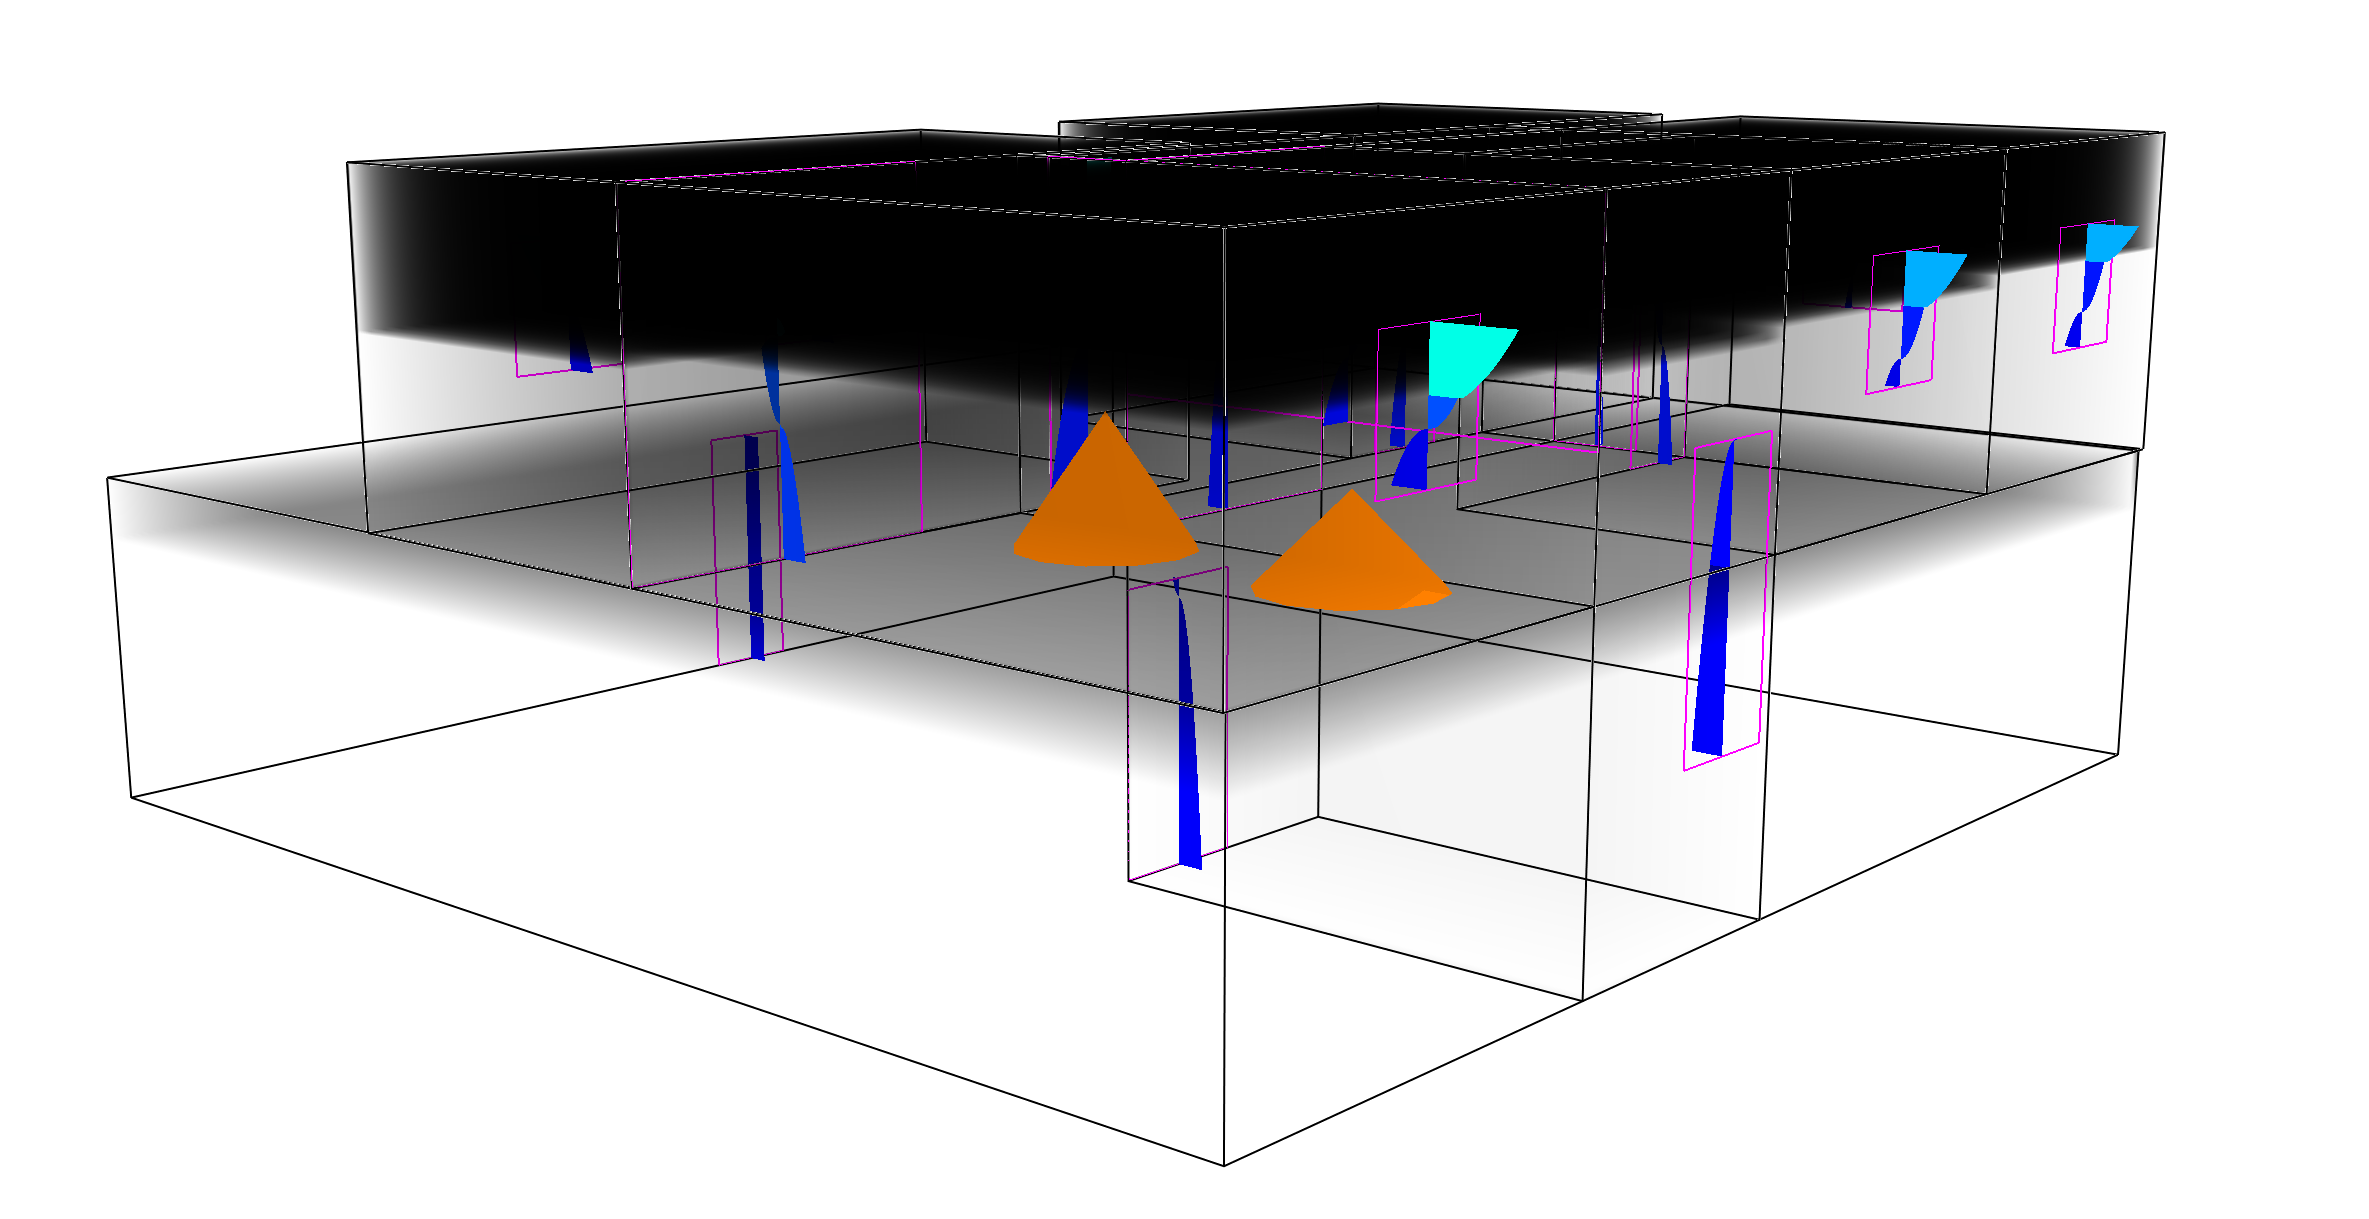
\includegraphics[width=6.5in]{FIGURES/Sample_Visualization.png}
\caption{Sample CFAST visualization of a single structure subject to a fire.}
\label{sample_visualization}
\end{figure}

Of course, if it is desired to study the impact of fires in a set of more than one specific building, the compartment geometry and placement could be defined by multiple individual buildings with the specific building chosen for an individual scenario chosen at random or from a distribution representing the population of each building type in the community under study.

The set of buildings for study can also be chosen from distributions of building and room characteristics. Figure \ref{sample_room_distribution} shows the distribution of the total floor area in a residence, the number of bedrooms in a residence depending on the total floor area, the total number of rooms given a certain number of bedrooms (here shown for residences from 1000~ft$^2$ to 1500~ft$^2$), all taken from the 2015 U.S. Housing Survey \cite{AHS2015}. Creating a compartment geometry from these data can be thought of as a six step process:

\begin{enumerate}
    \item randomly select the total floor area of the structure, Fig. \ref{sample_room_distribution}(a);
    \item randomly select the total number of bedrooms for a structure of the size chosen in step 1, Fig. \ref{sample_room_distribution}(b);
    \item randomly select the total number of rooms in the structure of the chosen size and number of bedrooms (Fig. \ref{sample_room_distribution}(c) shows a sample distribution for homes ranging from 1000~ft$^2$ to 1500~ft$^2$. Distributions for other home sizes are available in ref. \cite{AHS2015});
    \item determine room sizes based on a distribution of bedroom sizes, allocating left over space to the other rooms;
    \item connect compartments as desired (for example by randomly setting vents as open or closed between compartment pairs); and
    \item ensure that the resulting structure is realizable (This random approach to generating connections has a probability of resulting in a floorplan that cannot be instantiated in a single story. More technically, if the floorplan is thought of as a graph with the rooms as vertices and the connections as edges, some of the randomly generated graphs will be nonplanar for cases with more than four rooms. A planar graph is one that can be drawn on a piece of paper and none of the edges cross. The probability of generating a nonplanar floorplan increases as the number of rooms increases. In order to eliminate such nonphysical cases from the analysis, any randomly generated floorplan can be checked for planarity and rejected if necessary and replaced by a new randomly generated floorplan).
\end{enumerate}

\begin{figure}[p]
\begin{tabular*}{\textwidth}{c}
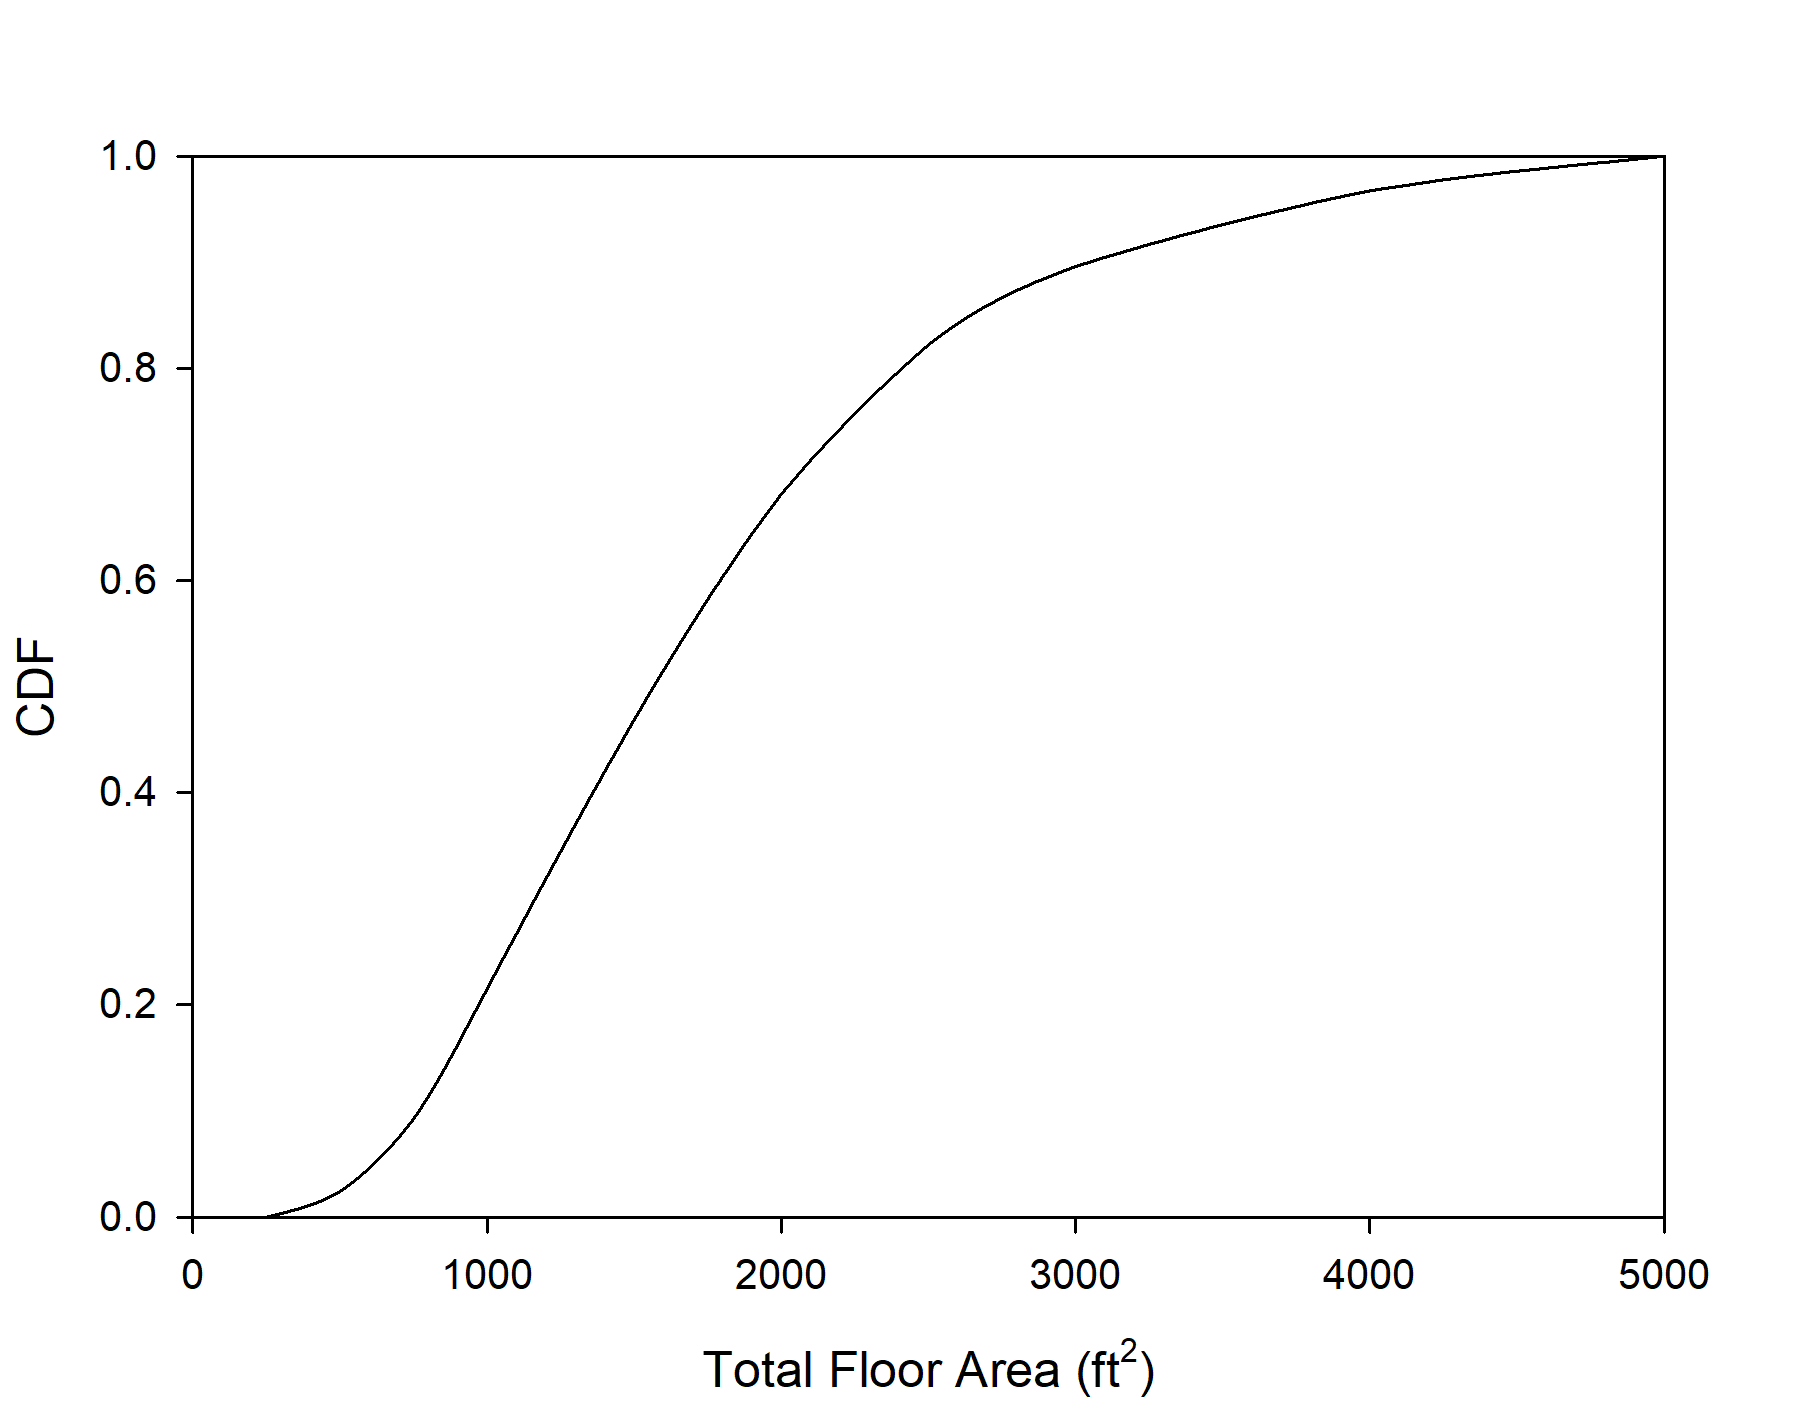
\includegraphics[height=2.5in]{FIGURES/Total_Floor_Area} \\
(a) Total Floor Area in a Residence \\
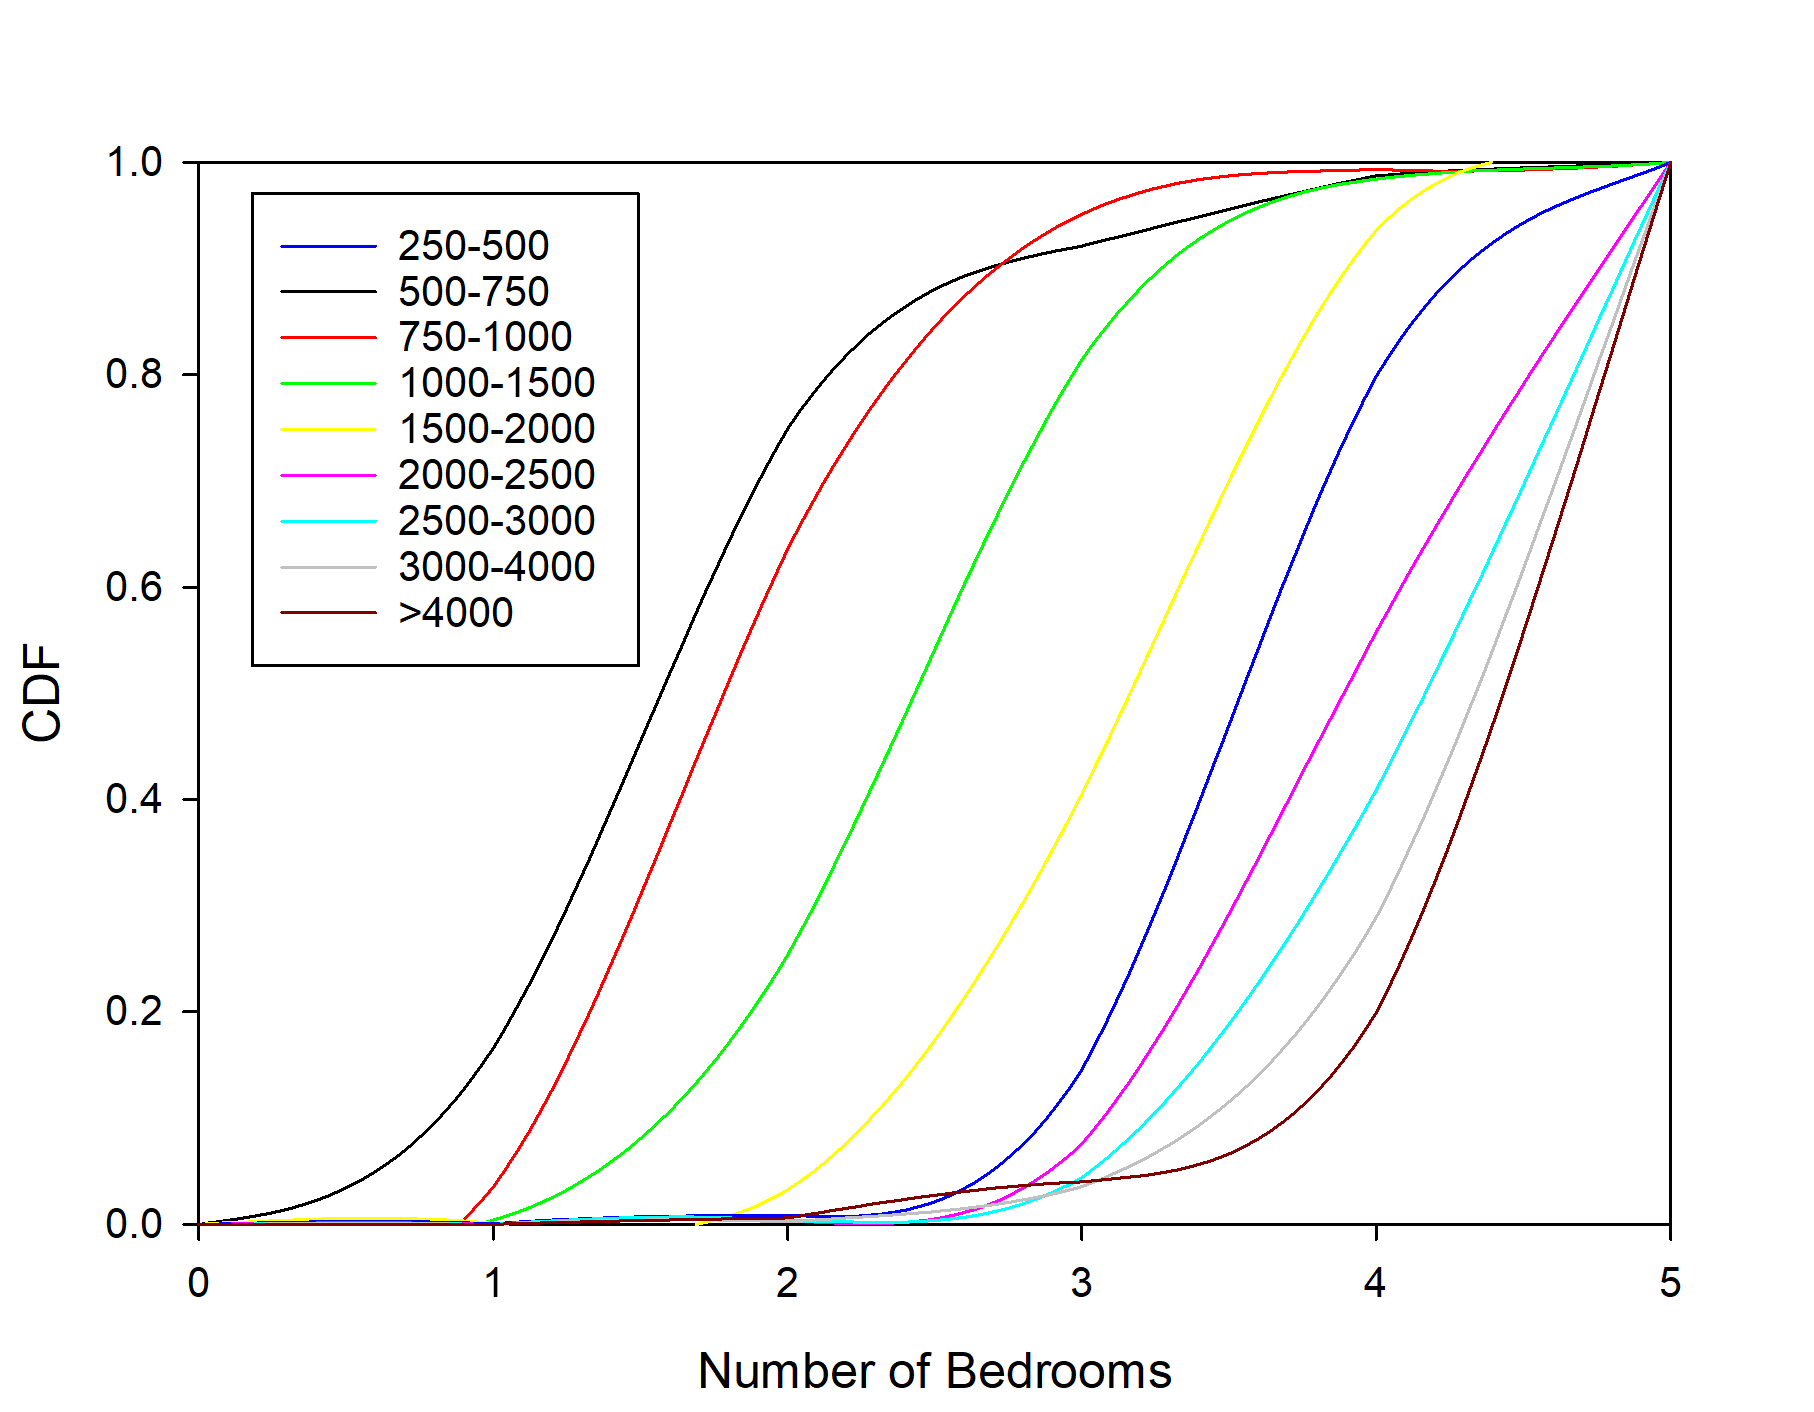
\includegraphics[height=2.5in]{FIGURES/Number_of_Bedrooms} \\
(b) Number of Bedrooms in a Residence as a Function of Total Floor Area \\
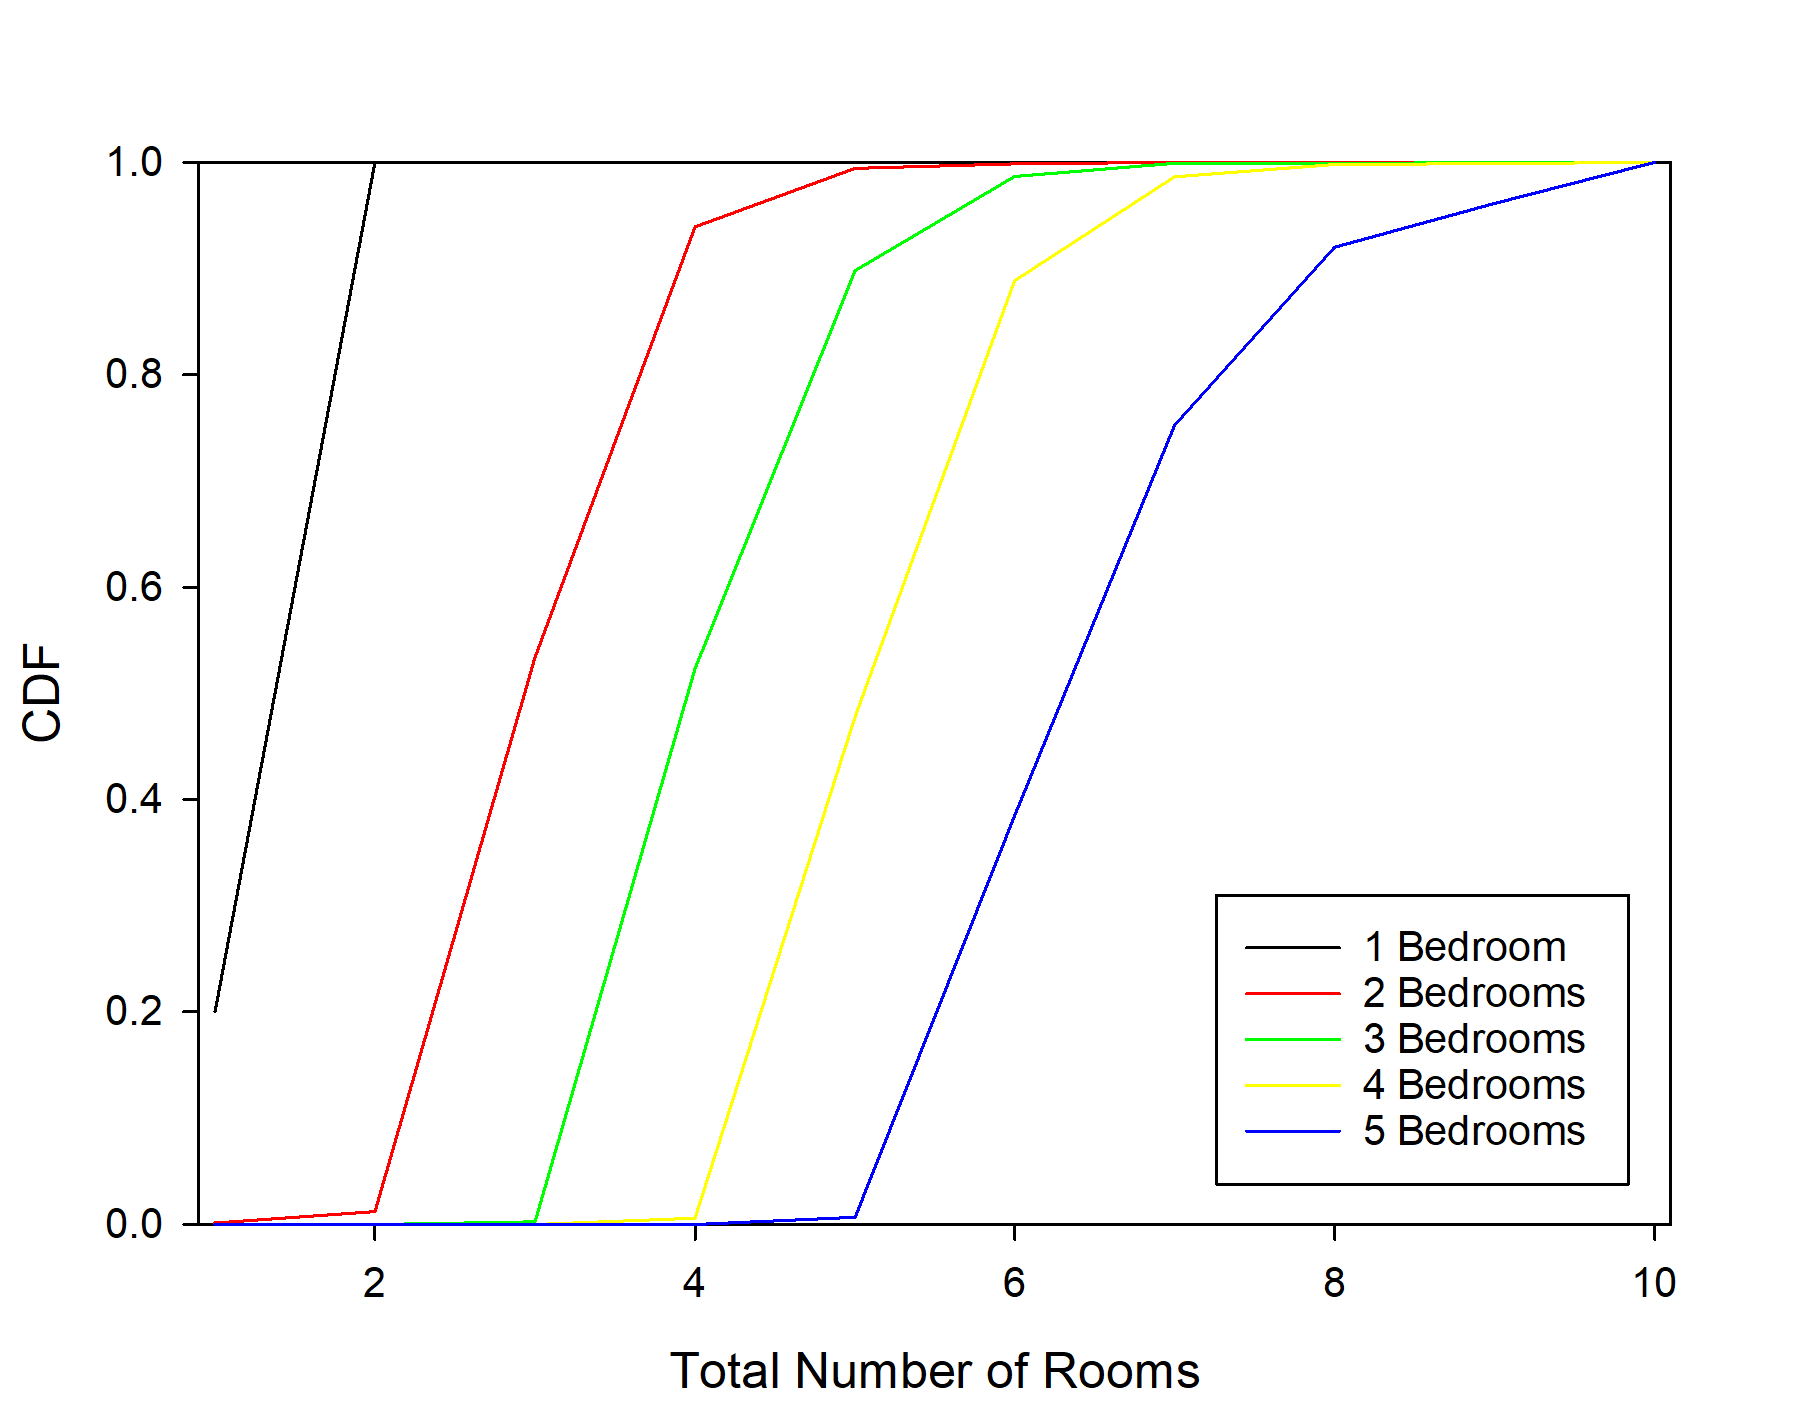
\includegraphics[height=2.5in]{FIGURES/Total_Rooms} \\
(c) Total Number of Rooms as a Function of the Number of Bedrooms in a Residence with  \\
1000 ft$^2$ - 1500 ft$^2$ of Total Floor Area  \\
\end{tabular*}
\caption[Cumulative Probability Distributions for Home Size, Number of Bedrooms and Total Number of Rooms]
{Example Cumulative Probability Distributions for Home Size, Number of Bedrooms and Total Number of Rooms (excluding Bathrooms) taken from the 2015 U.S. Housing Survey \cite{AHS2015}}
\label{sample_room_distribution}
\end{figure}

Other characteristics of the structure such as materials of construction, vent openings, fire definitions, measurement targets, sprinklers, and detection devices can be varied as desired for the problem being studied. Table \ref{tbl:distributable_variables} shows variables in the modeling that can be varied based on user-defined distributions \footnote{The content of this table follows the form of that used in B-Risk \cite{BranzFire}, adapted to be applicable to the calculational capabilities of the CFAST model.}.

\noindent
\begin{longtable}{@{\extracolsep{\fill}}|l|l|l|}
\caption[CFAST Inputs That Can be Varied Based on User-Defined Distributions]{CFAST Inputs That Can be Varied Based on User-Defined Distributions}
\label{tbl:distributable_variables} \\ \hline
\parbox{2in}{\bf Category}    & \parbox{2in}{\bf Input}  & \parbox{2in}{\bf Units} \\ \hline
\endfirsthead
\caption[]{Continued} \\ \hline
\parbox{2in}{\bf Category}    & \parbox{2in}{\bf Input}  & \parbox{2in}{\bf Units} \\ \hline
\endhead
Ambient Conditions      & Interior Temperature          & \degc                     \\
                        & Exterior Temperature          & \degc                     \\
                        & Relative Humidity             & \%                        \\ \hline
Thermal Properties      & Thermal Conductivity          & kW/(m~\degc)              \\
                        & Specific Heat                 & kJ/(kg~\degc)             \\
                        & Density                       & kg/m$^3$                  \\
                        & Default Thickness             & m                         \\
                        & Emissivity                    &                           \\ \hline
Compartments            & Width                         & m                         \\
                        & Depth                         & m                         \\
                        & Height                        & m                         \\
                        & Width Position                & m                         \\
                        & Depth Position                & m                         \\
                        & Height Position               & m                         \\
                        & Wall Leak Area Ratio          & m$^2$/m$^2$               \\
                        & Floor Leak Area Ratio         & m$^2$/m$^2$               \\ \hline
 Wall Vents             & Sill                          & m                         \\
                        & Soffit                        & m                         \\
                        & Width                         & m                         \\
                        & Initial Opening Fraction      & 0-1                       \\
                        & Open/Close Time               & s                         \\
                        & Final Opening Fraction        & 0-1                       \\
                        & Setpoint                      & s, \degc, or kW/m$^2$     \\
                        & Pre-Activation Fraction       & 0-1                       \\
                        & Post-Activation Fraction      & 0-1                       \\ \hline
 Ceiling / Floor Vents  & Cross-Sectional Area          & m$^2$                     \\
                        & Initial Opening Fraction      & 0-1                       \\
                        & Open/Close Time               & s                         \\
                        & Final Opening Fraction        & 0-1                       \\
                        & Setpoint                      & s, \degc, or kW/m$^2$     \\
                        & Pre-Activation Fraction       & 0-1                       \\ \hline
 Mechanical Vents       & From Compartment Area         & m$^2$                     \\
                        & From Compartment Height       & m                         \\
                        & To Compartment Area           & m$^2$                     \\
                        & To Compartment Height         & m                         \\
                        & Flow Rate                     & m$^3$/s                   \\
                        & Begin Dropoff                 & Pa                        \\
                        & End Dropoff                   & Pa                        \\
                        & Initial Opening Fraction      & 0-1                       \\
                        & Open/Close Time               & s                         \\
                        & Final Opening Fraction        & 0-1                       \\
                        & Setpoint                      & s, \degc, or kW/m$^2$     \\
                        & Pre-Activation Fraction       & 0-1                       \\
                        & Post-Activation Fraction      & 0-1                       \\
                        & Filter Efficiency             & \%                        \\
                        & Begin Filtering Time          & s                         \\ \hline
Fires                   & \multicolumn{2}{|c|}{See Section \ref{Fire_Scenarios}}    \\ \hline
Targets                 & Width Target Position         & m                         \\
                        & Depth Target Position         & m                         \\
                        & Height Target Position        & m                         \\
                        & Width Normal Vector           & 0-1                       \\
                        & Depth Normal Vector           & 0-1                       \\
                        & Height Normal Vector          & 0-1                       \\
                        & Target Points To              & Selection List            \\
                        & Thickness                     & m                         \\
                        & Internal Temperature Location & m                         \\ \hline
Detection / Suppression & Width Position                & m                         \\
                        & Depth Position                & m                         \\
                        & Height Position               & m                         \\
                        & Activation Temperature        & \degc                     \\
                        & Activation Obscuration        & \%/m                      \\
                        & RTI                           & (m~s)$^{1/2}$             \\
                        & Spray Density                 & m/s                       \\ \hline
\end{longtable}

\clearpage

\section{Fire Scenarios}
\label{Fire_Scenarios}

\subsection{Individual Variables}

The quantitative definition of fires is arguably the most important \cite{Babrauskas:1992} and complex of all the inputs in any fire modeling scenario. It includes specification of the fire location, fuel composition, ignition criterion, heat release rate, burning area, and species yields, most of which can vary with time over the course of the fire.

\noindent
\begin{longtable}{@{\extracolsep{\fill}}|l|l|l|}
\caption[CFAST Fire Inputs That Can be Varied Based on User-Defined Distributions]{CFAST Fire Inputs That Can be Varied Based on User-Defined Distributions}
\label{tbl:fire_variables} \\ \hline
\parbox{2in}{\bf Category}    & \parbox{2in}{\bf Input}  & \parbox{2in}{\bf Units} \\ \hline
\endfirsthead
\caption[]{Continued} \\ \hline
\parbox{2in}{\bf Category}    & \parbox{2in}{\bf Input}  & \parbox{2in}{\bf Units} \\ \hline
\endhead
Fire Location           & Compartment                   & Selection List                \\
                        & Width Position                & m                             \\
                        & Depth Position                & m                             \\ \hline
Fuel Composition        & Carbon Molecules              & $\geq$ 0                      \\
                        & Hydrogen Molecules            & $\geq$ 0                      \\
                        & Oxygen Molecules              & $\geq$ 0                      \\
                        & Nitrogen Molecules            & $\geq$ 0                      \\
                        & Chlorine Molecules            & $\geq$ 0                      \\
                        & Heat of Combustion            & kJ/kg                         \\
                        & Radiative Fraction            & 0 - 1                         \\ \hline
Ignition Criteria       & Ignition Criterion            & Selection List                \\
                        & Setpoint                      & s, \degc, or kW/m$^2$         \\ \hline
Time Histories          & \multicolumn{2}{|c|}{See Section \ref{Fire_Time_Histories}}   \\ \hline
\end{longtable}

\subsection{Time Histories}
\label{Fire_Time_Histories}

Some examples of different definitions of time histories go here.

\noindent
\begin{longtable}{@{\extracolsep{\fill}}|l|l|l|}
\caption[CFAST Fire Time Histories That Can be Varied Based on One or More User-Defined Distributions]{CFAST Fire Time Histories That Can be Varied Based on One or More User-Defined Distributions}
\label{tbl:fire_variables} \\ \hline
\parbox{2in}{\bf Category}    & \parbox{2in}{\bf Input}  & \parbox{2in}{\bf Units} \\ \hline
\endfirsthead
\caption[]{Continued} \\ \hline
\parbox{2in}{\bf Category}    & \parbox{2in}{\bf Input}  & \parbox{2in}{\bf Units} \\ \hline
\endhead
Time Histories          & HRR                           & kW                        \\
                        & Fire Height                   & m                         \\
                        & Fire Area                     & m$^2$, >0                 \\
                        & CO Yield                      & kg CO/kg fuel             \\
                        & Soot Yield                    & kg Soot/kg fuel           \\
                        & HCN Yield                     & kg HCN/kg fuel            \\ \hline
\end{longtable}

\section{Defining Data for Analysis}

Choosing modeling results for analysis depends on the goals of the hazard analysis and the particular technology under study. In the most general sense, this means understanding what results are indicative of improved fire safety. This is not a cost benefit analysis, which is a superset of this analysis and outside the scope of this project. To improve fire safety generally means reducing the deaths and injuries due to a fire. So, the goal is to identify which variables, that can be calculated, would give an indication that a new technology, in our case the new smoke alarm technology, will reduce deaths and injuries.

\section{Examples}

\subsection{Example 1: Impact of new detector standard}

\subsection{Example 2: Impact of inner liners on residential upholstered furniture fires}

\subsection{Example 3: Impact of periodically active wireless detectors}

%
%---------------------User's Guide----------------------------------
%

\chapter{CData User's Guide}
The CData program has several functions. One of them is as a PreProcessor used to create a set of data files that CFAST runs to generate data for an analysis. This chapter discusses how the PreProcessor works with some simple examples to demonstrate certain aspects of the system. First is an overview of the basic philosophy behind the PreProcessor. Section \ref{commands_section} discusses all the namelist commands that work in the PreProcessor. The final section discusses the significant issue of storage, which can limit on the size of the analysis that can be done.

\section{Basic Philosophy}

\section{PreProcessor}

\subsection{Commands}
\label{commands_section}
Each subsection will discuss one namelist and what each of the parameters do. The tables presented in each subsection are combined in Appendix \ref{preprocessor_reference}  to serve as a refence for commands.

\subsubsection{Namelist DUMP}

\subsubsection{Namelist MHDR}

\subsubsection{Namelist MRND}

\subsubsection{Namelist MFLD}

\subsubsection{Namelist MFIR}

\section{Running CFAST}

\subsection{Running on Different Operating Systems}

\subsection{The Question of Storage}

\section{Generating Statistics}

\subsection{Accumulator}

\subsection{Statistics}

\subsubsection{Determining If Enough Runs Have Been Made}

\subsubsection{Correlation Trees}

%
%-------------------------Analysis of Data-------------------------------------------
%

\chapter{Analysis of Data}

\section{General Analysis}

\section{Examples}

\subsection{Example 1}

\subsection{Example 2}

\subsection{Example 3}

%
% -------------------  Summary ------------------------
%

\chapter{Summary and Future Work}

\bibliography{../Bibliography/CFAST_refs}

\appendix
\addcontentsline{toc}{chapter}{Appendices}

%
% -------------------  Nomenclature ------------------------
%

\chapter{Nomenclature}
\label{nomenclature}

Note that the units associated with a given symbol are sometimes changed upon input to and output from the program. In particular, temperatures are typically input in degrees Celsius, converted to Kelvin, and then converted back to Celsius on output. Energy units involving Joules or Watts are typically input as kJ or kW, converted to J or W, then converted back to kJ or kW.

\begin{center}
\begin{longtable}{p{1in}  p{5.5 in}}

$A$                 & area, m$^2$ \\
\end{longtable}

\end{center}

\chapter{PreProcessor Reference}
\label{preprocessor_reference}
Each subsection will discuss one namelist and what each of the parameters does. The tables presented in each subsection are combined in Appendix XXX  to serve as a refence for commands.

\section{Namelist DUMP}

\section{Namelist MHDR}

\section{Namelist MRND}

\section{Namelist MFLD}

\section{Namelist MFIR}

\section {Namelist MSTT}
\chapter{Supplemental Material}

\chapter{Change Log}

\label{last_page}

\end{document}
